\documentclass[10pt]{beamer}

\usetheme[progressbar=frametitle]{metropolis}

\usepackage[absolute,overlay]{textpos}
\usepackage{booktabs}
\usepackage[scale=2]{ccicons}
%\usepackage[brazilian]{babel}
%\usepackage[T1]{fontenc}    % Selecao de codigos de fonte.
\usepackage[utf8]{inputenc} 

\usepackage{pgfplots}
\usepgfplotslibrary{dateplot}

\usepackage{xspace}
\newcommand{\themename}{\textbf{\textsc{metropolis}}\xspace}

\title{Aplicando a Teoria Mie-Debye para Caracterização de Parâmetros Físicos \\em Pinças Óticas}
\subtitle{Defesa de Dissertação de Mestrado}
\date{\today}
\author{Arthur Luna da Fonseca \\Orientadores: Paulo Américo Maia Neto, Rafael de Sousa Dutra}
\date{10 de Setembro de 2019}
\institute{Instituto de Física - Universidade Federal do Rio de Janeiro}
\titlegraphic{\hfill
\includegraphics[height=2.cm]{../logo_ufrj}}

\begin{document}

\maketitle

%%%%%%%%%%%%%%%%%%%%%%%%%%%%%%%%%%%%%%%%%%%%%%%%%%%%%%%%%%%%%%%%%%%%%%%%%%%%%%%%%%%%%%%%%%%%%%%%%

\begin{frame}{Conteúdo}
  \setbeamertemplate{section in toc}[sections numbered]
  \tableofcontents[hideallsubsections]
\end{frame}

%%%%%%%%%%%%%%%%%%%%%%%%%%%%%%%%%%%%%%%%%%%%%%%%%%%%%%%%%%%%%%%%%%%%%%%%%%%%%%%%%%%%%%%%%%%%%%%%%

\section{Introdução}

%%%%%%%%%%%%%%%%%%%%%%%%%%%%%%%%%%%%%%%%%%%%%%%%%%%%%%%%%%%%%%%%%%%%%%%%%%%%%%%%%%%%%%%%%%%%%%%%%

\begin{frame}[fragile]{Introdução}
      \begin{center}
          \metroset{block=fill}
          \begin{exampleblock}{Objetivo}
            Caracterização de parâmetros na pinça ótica:\\
            \hspace{1mm}\\
            \hspace{4mm}$\rightarrow$Teoria MDSA+ para pinças óticas:\\
            \hspace{7mm}$\rightarrow$Correções de aberrações óticas na teoria MDSA $\rightarrow$Astigmatismo.\\
            \hspace{7mm}$\rightarrow$Espalhamento Mie $\rightarrow$Parâmetro de absorção da microesfera.\\
            \hspace{1mm}\\
            \hspace{4mm}$\rightarrow$Cálculo numérico usando a teoria MDSA+:\\
            \hspace{7mm}$\rightarrow$Simulação do experimento de transferência de momento angular na pinça ótica.\\
            \hspace{7mm}$\rightarrow$Cálculos da posição de equilíbrio da esfera variando o parâmetro de absorção.
          \end{exampleblock}
      \end{center}
\end{frame}

%%%%%%%%%%%%%%%%%%%%%%%%%%%%%%%%%%%%%%%%%%%%%%%%%%%%%%%%%%%%%%%%%%%%%%%%%%%%%%%%%%%%%%%%%%%%%%%%%

\begin{frame}[fragile]{Introdução}

Introdução à teoria de pinças óticas: \\
    \begin{center}
        Modelagens da pinça ótica: interação de um campo (feixe) com o objeto espalhador (esfera pinçada).

        Campo: feixe fortemente focalizado.

        Objeto espalhador: simetria esférica $\rightarrow$ espalhamento Mie.

        

    \end{center}

\end{frame}

\begin{frame}[fragile]{Regimes de tamanhos do objeto espalhador.}

Dois regimes distintos: \\
    \begin{center}
        Regime Rayleigh: raio da esfera muito menor que o comprimento de onda do feixe ($a<<\lambda$).

        Aproximamos a esfera por um dipolo induzido:
        \begin{equation}
        {\mathbf F} = \frac{1}{2}\nabla({\mathbf p}\cdot{\mathbf E})=\frac{1}{2}\nabla(\alpha{\mathbf E}^2).
        \end{equation}

        Força aponta para região de maior intensidade do campo. Para o feixe fortemente focalizado, a região de maio intensidade é o foco.

    \end{center}
.
\end{frame}

\begin{frame}[fragile]{Regimes de tamanhos do objeto espalhador.}

    \begin{center}
        Regime de ótica geométrica: raio da esfera muito mairo que o comprimento de onda do feixe ($a>>\lambda$).

        Ignorando efeitos de reflexão e de absorção, raios diametralmente\\opostos transferem momento para esfera na direção do foco.
        %
        \begin{picture}(320,250)
        \put(190,95){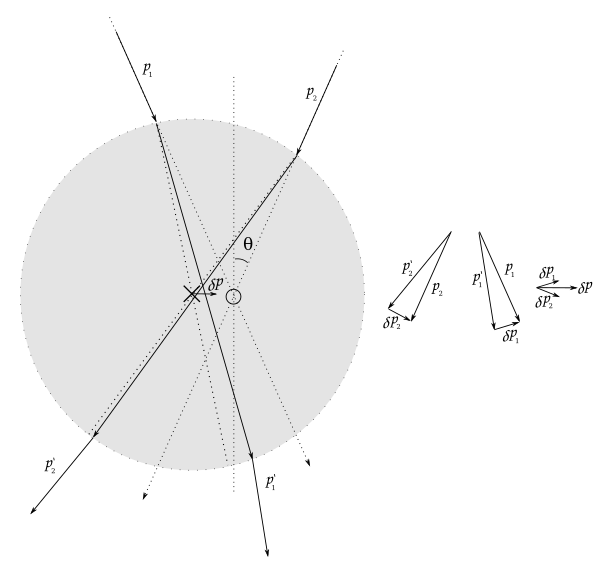
\includegraphics[scale=.40]{../geom_lateralIV}}
        \end{picture}

        \begin{picture}(320,250)
        \put(-17,332){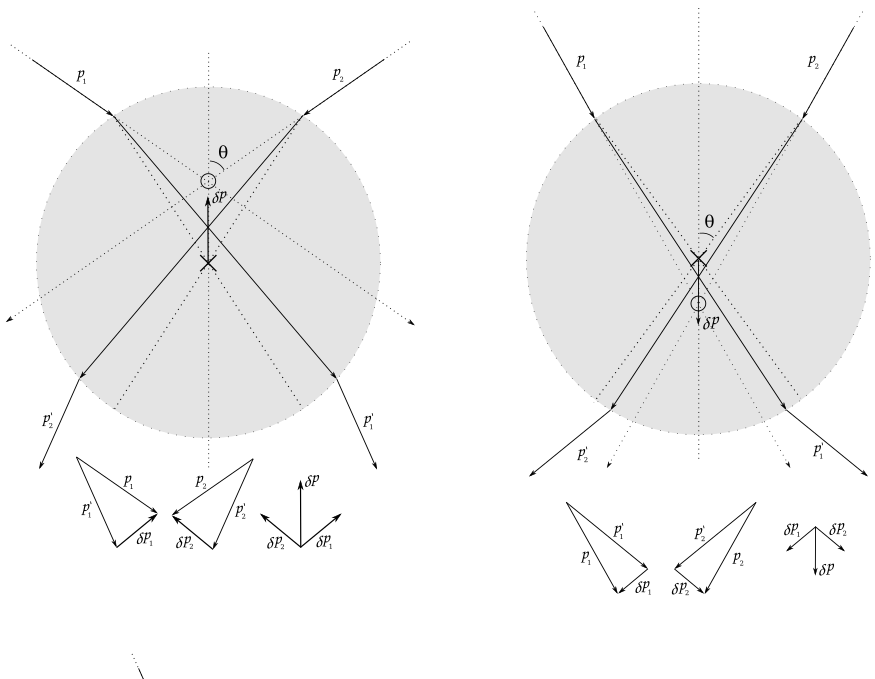
\includegraphics[scale=.38]{../geom_foco_axialIII}}
        \end{picture}
        %
        


    \end{center}

\end{frame}

\begin{frame}[fragile]{Regimes de tamanhos do objeto espalhador.}

    \begin{center}
        A posição de equilíbrio não necessariamente é no foco, \\pois a reflexão (a) transfere momento na direção normal ao plano tangente ao ponto de reflexão na esfera,\\enquanto a absorção (b) transfere na direção da propagação do raio:
        %
        \begin{picture}(320,250)
        \put(27,90){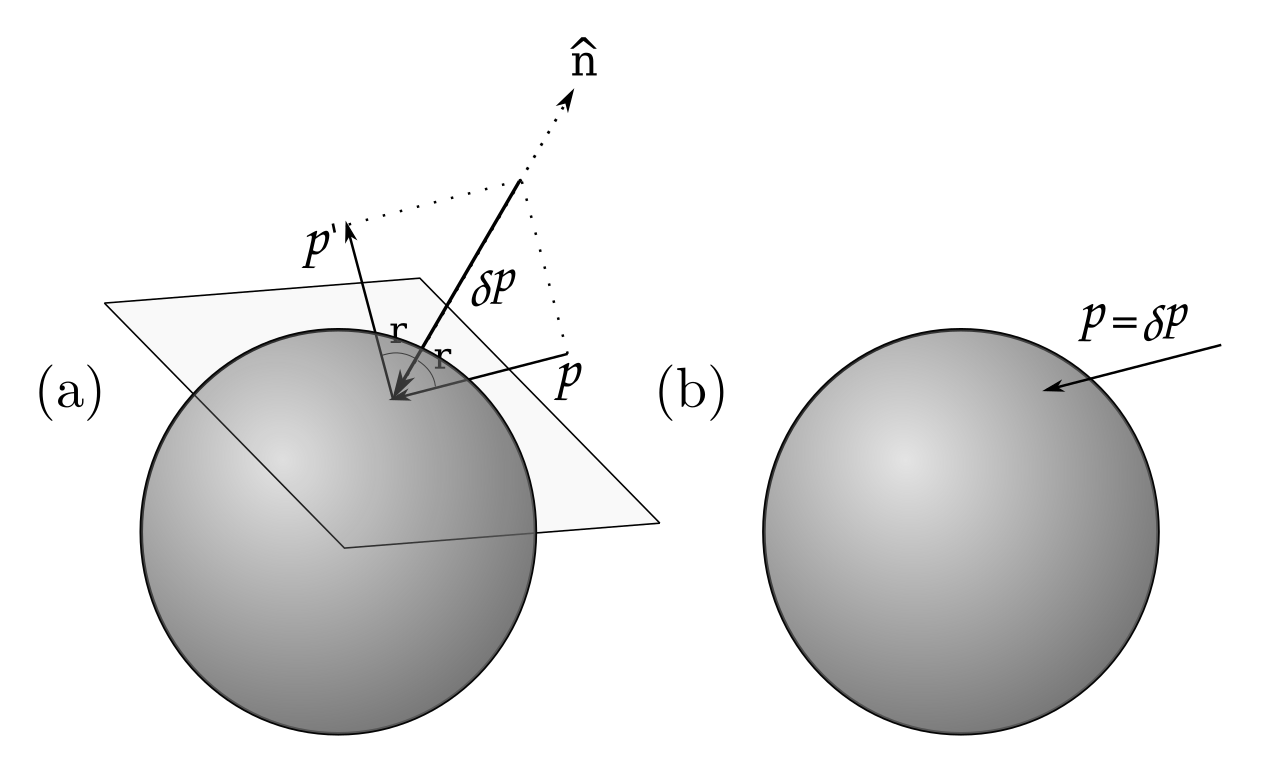
\includegraphics[scale=.25]{../reflex_absorII}}
        \end{picture}

    \end{center}

\end{frame}


\begin{frame}[fragile]{Introdução ao modelo MDSA.}

    \begin{center}
        O modelo Mie-Debye para a pinça ótica é um modelo exato para o espalhamento por uma esfera de um campo fortemente focalizado (por uma objetiva).

        O modelo para o campo foi desenvolvido por Richards e Wolf, baseado em uma proposição de Debye para um campo escalar produzido por uma objetiva de alta abertura numérica.
        
        O campo é expresso como uma superposição de ondas planas onde os vetores $\mathbf{k}(\theta_k,\phi_k)$ formam um cone de meia abertura $\theta_0$ no espaço de momento:
        %
        \begin{equation}
        \mathbf{E}_{IN}=\int\limits_0^{\theta_0} d\theta_k \sin\theta_k \int\limits_0^{2\pi} d\phi_k\sqrt{\sin\theta_k} e^{i\mathbf{k}\cdot\mathbf{r}}\hat{\varepsilon}_k,
        \label{RichWolf}
        \end{equation}

        onde o termo $\sqrt{\sin\theta_k}$ vem da condição de seno de Abbe ($f^2\sin^2\theta_k=\rho^2$) que as objetivas de alta abertura numérica satisfazem.

    \end{center}

\end{frame}

\begin{frame}[fragile]{Introdução ao modelo MDSA.}

    \begin{center}
        Para encontrarmos os campos espalhados pela esfera, calculamos os potenciais de Debye do campo incidente para cada caso de polarização circular, que são definidos por:
        %
        \begin{equation}
        \Pi^{E}=\sum\limits_{J} \Pi^{E}_J=\sum\limits_{J}\frac{ ({\mathbf r}\cdot{\mathbf E })_J }{J(J+1)} \qquad e\qquad \Pi^{M}=\sum\limits_{J} \Pi^{M}_J=\sum\limits_{J}\frac{ ({\mathbf r}\cdot{\mathbf H })_J }{J(J+1)} .
        \end{equation}

        O somatório em $J$ denota a expansão do campo em multipolos. Cada multipolo do campo incidente será espalhado com uma amplitude, dada pelos coeficiente de Mie $a_j$ (para os multipolos elétricos) e $b_j$ (para o multipolo magnético).

    \end{center}

\end{frame}

\begin{frame}[fragile]{Introdução ao modelo MDSA.}

    \begin{center}
        Para introduzirmos o efeito causado pelo perfil do feixe paraxial incidente na objetiva, inserimos a amplitude de campo em cada ponto da entrada da objetiva na equação \ref{RichWolf}:
        %
        \begin{equation}
        \mathbf{E}_{IN}=\int\limits_0^{\theta_0} d\theta_k \sin\theta_k \int\limits_0^{2\pi} d\phi_k\sqrt{\sin\theta_k} e^{i\mathbf{k}\cdot\mathbf{r}} e^{-\frac{f^2\sin^2\theta_k}{\omega_0^2}} \hat{\varepsilon}_k.        
        \end{equation}

        O caso de um feixe elipticamente polarizado é obtido tomando o feixe na entrada da objetiva como uma superposição de ondas circularmente polarizadas:
        \begin{equation}
        \hat{\varepsilon}_k = \sum \limits_{\sigma = +1,-1} \frac{1 - ie^{-2i\sigma \psi}}{2} \hat{\bf{\epsilon}}_\sigma .     
        \end{equation}

    \end{center}

\end{frame}


\begin{frame}[fragile]{Introdução ao modelo MDSA.}

    \begin{center}
        Depois que o feixe focalizado é produzido pela objetiva, ele incide no porta amostra, passando por uma interface de vidro e água. Algumas objetivas de alta abertura numérica são de imersão em óleo, o que faz com que haja um efeito de aberração esférica que deve ser levado em conta no modelo.
        %
        \begin{picture}(320,250)
        \put(45,90){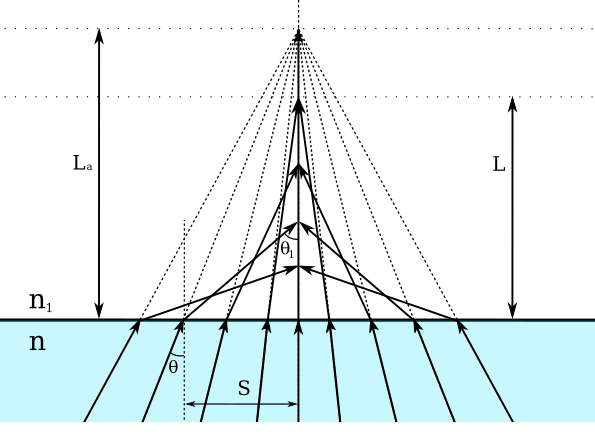
\includegraphics[scale=.6]{../aberracao_esf4}}
        \end{picture}
    \end{center}

\end{frame}


\begin{frame}

    \begin{center}
        Esse efeito insere uma fase em cada componente de onda plana do campo, de acordo com seu ângulo de incidência, que pode ser obtida através da lei de Snell:
        %
        \begin{equation}
        \Psi(z,\theta) = k\left( -\frac{L}{N}\cos\theta + N L\cos\theta_1 \right).
        \end{equation}

        Também haverá reflexão nessa interface, e portanto devemos levar a amplitude de transmissão de Fresnel em consideração:
        %
        \begin{equation}
        T(\theta)=\frac{2\cos\theta}{\cos\theta + N\cos\theta_1}.     
        \end{equation}
    \end{center}

\end{frame}

\begin{frame}[fragile]{Introdução ao modelo MDSA.}

    \begin{center}
        Outras aberrações óticas também podem ser incluidas no modelo usado o formalismo de Zernike, que utiliza um conjunto de polinômios que formam uma base para descrever as fases de cada aberração ótica de um feixe. Os polinômios de Zernike formam uma base ortonormal no círculo unitário, o que nos permite descrever qualquer aberração ótica do sistema.\\
        Nos experimentos realizados pelo grupo, a aberração de interesse é o astigmatismo.

        \begin{picture}(320,250)
        \put(34,132){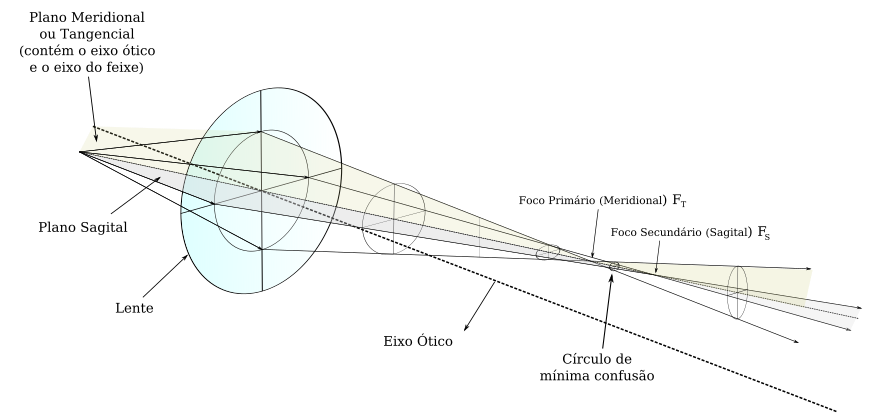
\includegraphics[scale=.4]{../feixe_astig}}
        \end{picture}
    \end{center}

\end{frame}

\begin{frame}

    \begin{center}
        A fase associada ao astigmatismo é:
        %
        \begin{equation}
        \Phi_{astigmatismo}(\theta,\phi) = 2\pi A_{ast}\left( \frac{\sin\theta}{\sin\theta_0} \right)^2\cos2(\phi - \varphi_a),
        \end{equation}
        onde o círculo unitário foi definido como o círculo formado pela entrada da objetiva, que tem raio $R_p=f\sin\theta_0$ (pela condição do seno de Abbe).

        O parâmetro $A_{ast}$ é o chamado parâmetro de astigmatismo. Um dos objetivos do trabalho é a determinação desse parâmetro por meio de ajustes do modelo.

    \end{center}

\end{frame}

\begin{frame}

    \begin{center}
        Finalmente, expressamos a força em termos do fator de eficiência $\mathbf{Q}$:
        %
        \begin{equation}
        {\mathbf Q} = \frac{\left<{\mathbf F}\right>}{n_1 P/c}= |a_+|^2{\mathbf Q}^{(\sigma +)} + |a_-|^2{\mathbf Q}^{(\sigma -)} + {\mathbf Q}^{({\it cross},+-)} + {\mathbf Q}^{({\it cross},-+)}.
        \end{equation}
        
        onde $n_1$ é o índice de refração do meio em que a microesfera está inserida e $P$ é a potência do laser.

        O fator de eficiência na direção $z$ será usado para calcular a posição de equilíbrio axial nas simulações. Uma das grandezas medidas no experimento são as constante eláticas $\kappa_\rho$ e $\kappa_\phi$, definidas como:

        \begin{equation}
        \kappa_\rho=-\frac{n_1 P}{c}\frac{\partial Q_\rho}{\partial \rho}\Big{|}_{\rho=0, \thinspace z=z_{eq}} \qquad, \qquad \kappa_\phi=\frac{n_1 P}{c}\frac{\partial Q_\phi}{\partial \rho}\Big{|}_{\rho=0, \thinspace z=z_{eq}}.
        \end{equation}
%
    \end{center}

\end{frame}

%%%%%%%%%%%%%%%%%%%%%%%%%%%%%%%%%%%%%%%%%%%%%%%%%%%%%%%%%%%%%%%%%%%%%%%%%%%%%%%%%%%%%%%%%%%%%%%%%

\section{Simulação do experimento de transferência de momento angular}

%%%%%%%%%%%%%%%%%%%%%%%%%%%%%%%%%%%%%%%%%%%%%%%%%%%%%%%%%%%%%%%%%%%%%%%%%%%%%%%%%%%%%%%%%%%%%%%%%

\begin{frame}[fragile]{Experimento de transferência de momento angular}
    \begin{center}
        Para entender a simulação, é necessário discutir o experimento que mede o torque ótico na microesfera. Começamos pela geração do feixe paraxial na mesa ótica, ilustrada a seguir:

        \begin{picture}(320,250)
        \put(34,90){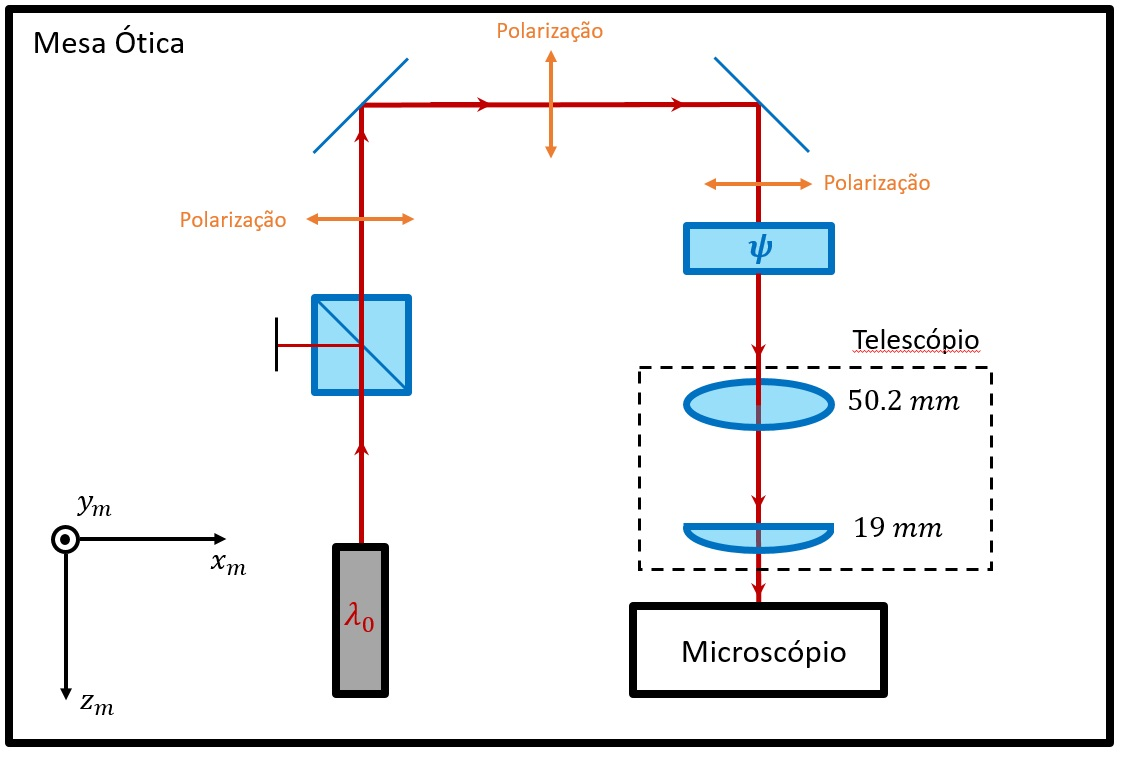
\includegraphics[scale=.21]{../fig/setup}}
        \end{picture}

    \end{center}
\end{frame}

%%%%%%%%%%%%%%%%%%%%%%%%%%%%%%%%%%%%%%%%%%%%%%%%%%%%%%%%%%%%%%%%%%%%%%%%%%%%%%%%%%%%%%%%%%%%%%%%%

\begin{frame}[fragile]{Experimento de transferência de momento angular}
    \begin{center}
        Dessa forma, o feixe entra no microscópio com polarização definida e cintura bem determinada, parâmetros estes que são de grande importância para simulação.

        O feixe, então, é refletido por um espelho dicróico, passa pela objetiva e incide no porta amostra, onde há a solução de microesfera.

        Através do espelho dicróico podemos tomar as imagens da amostra com uma câmera (CMOS).

    \end{center}
\end{frame}


\begin{frame}[fragile]{Experimento de transferência de momento angular}
    \begin{center}

        \begin{picture}(310,250)
        \put(10,40){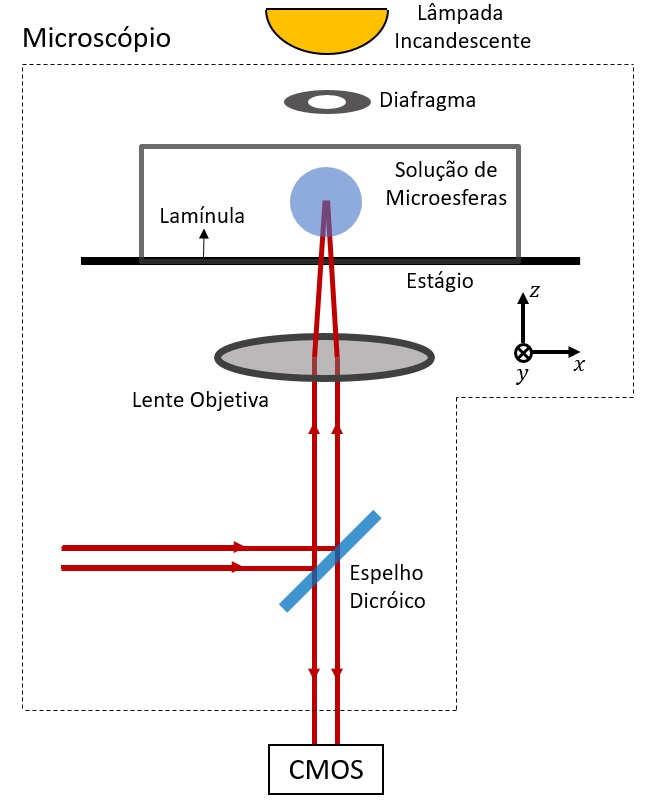
\includegraphics[scale=.35]{../fig/microscopio}}
        \end{picture}

        \begin{picture}(320,250)
        \put(185,350){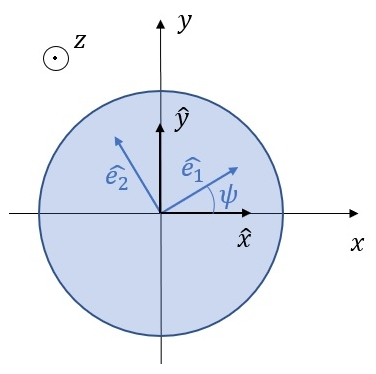
\includegraphics[scale=.33]{../fig/QWP}}
        \end{picture}

    \end{center}
\end{frame}

\begin{frame}[fragile]{Experimento de transferência de momento angular}
    \begin{center}
        O procedimento do experimento começa encostando a microesfera na lamínula. Em seguida, abaixa-se o estágio popr uma distância bem determinada e o deslocamos na direção de $\hat{x}$ com velocidades bem definidas. A força de arrasto do líquido (força de Stokes) é proporcional à velocidade de deslocamento do fluido, e desloca a microesfera na mesma direção e sentido. 

        Assumimos que as forças que são realizadas na esfera pelo feixe ao ser deslocada do eixo em que $\rho=0$ são harmônicas. 

    \end{center}
\end{frame}

\begin{frame}

    \begin{center}
        Teremos, então, no equilíbrio de forças, $\vec{F_\phi}+\vec{F_\rho}=-\vec{F_s}$. Observando a projeção na direção $y$, onde $\vec{F_s}\cdot\hat{y}=0$ e $F_\rho\sin\phi = F_\phi\cos\phi$:
        %
        \begin{equation}
        \frac{F_\phi}{F_\rho} = \tan\phi \approx \phi,
        \end{equation}
        
        onde $\phi$ é a coordenada angular da popsição de equilíbrio. Como as forças óticas são lineares, temos:
        %
        \begin{equation}
        \frac{\kappa_\phi}{\kappa_\rho} \approx \phi.
        \end{equation}
%
    \end{center}

\end{frame}

\begin{frame}[fragile]{Experimento de transferência de momento angular}
    \begin{center}
        É importante destacar que o ângulo $\phi$ não varia com a velocidade. Podemos ver abaixo o diagrama de forças da microesfera deslocada do eixo, e a reta formada pelas posições de equilíbrio de várias velocidades do estágio diferentes.

        \begin{picture}(310,250)
        \put(-22,130){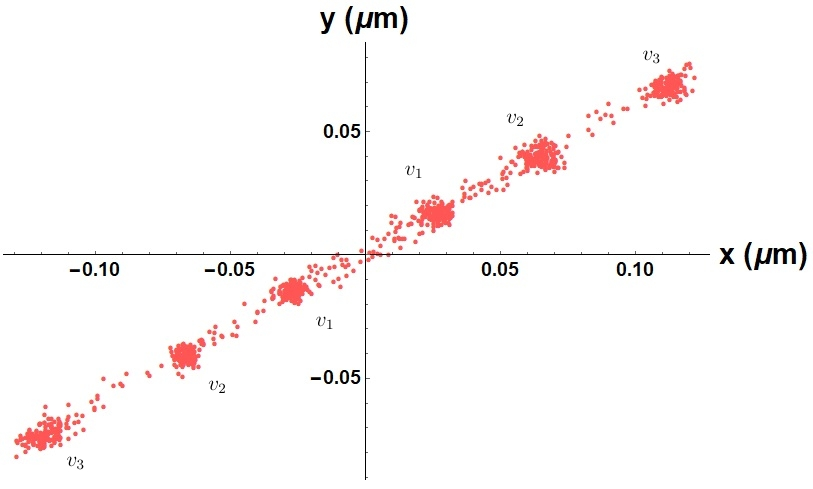
\includegraphics[scale=.2]{../fig/pos_eq_phi}}
        \end{picture}

        \begin{picture}(320,250)
        \put(145,385){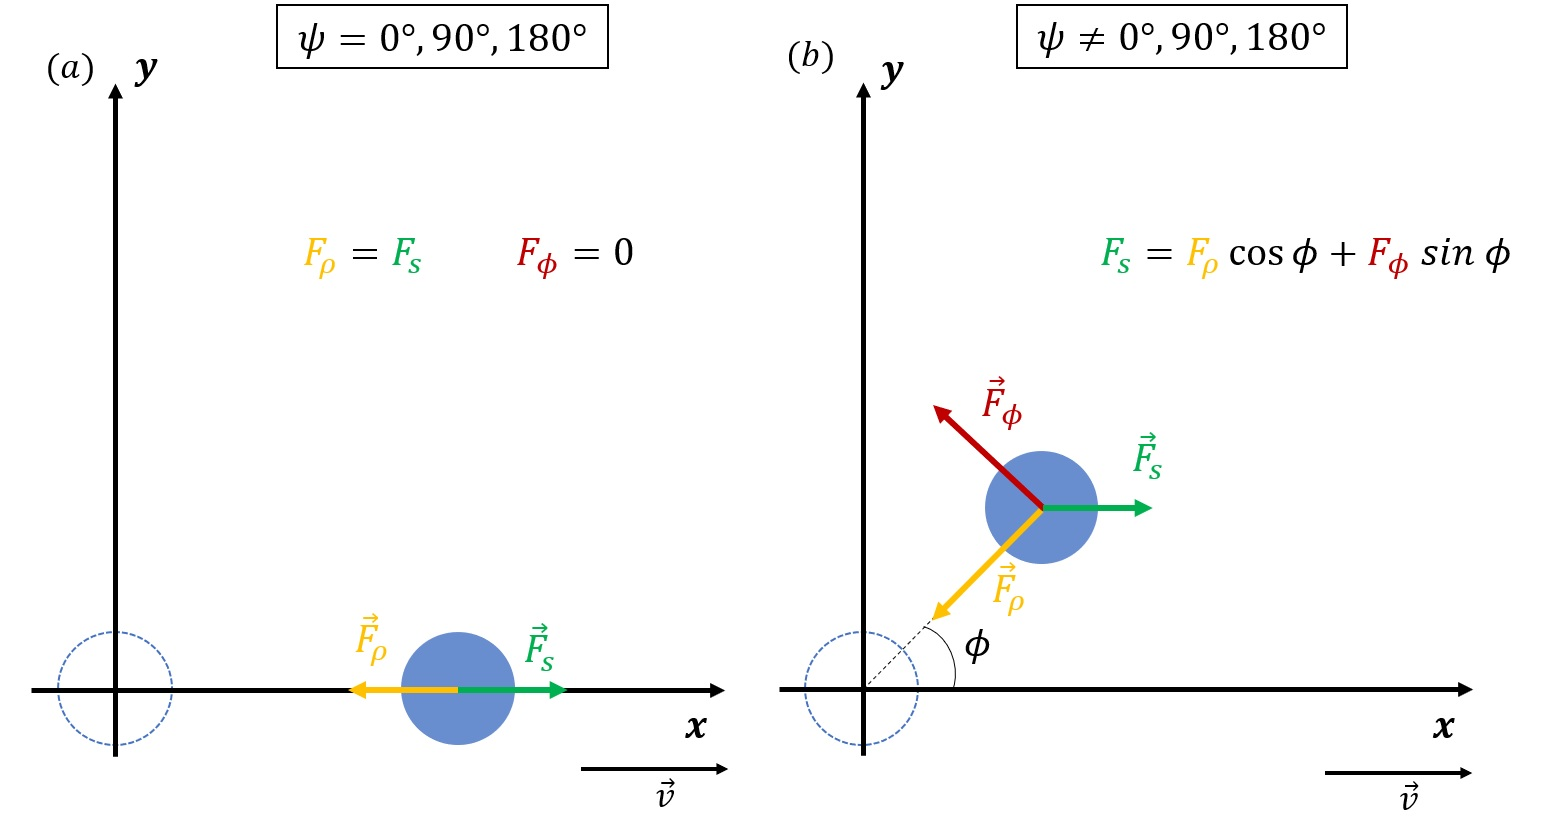
\includegraphics[scale=.16]{../fig/forcas_estagio}}
        \end{picture}

    \end{center}
\end{frame}

%%%%%%%%%%%%%%%%%%%%%%%%%%%%%%%%%%%%%%%%%%%%%%%%%%%%%%%%%%%%%%%%%%%%%%%%%%%%%%%%%%%%%%%%%%%%%%%%%

\begin{frame}[fragile]{Simulação do experimento}

    \begin{center}

        Para iniciar a simulação, calcula-se a posição do foco do feixe em relação à interface, quando a microesfera está encostada na lamínula e em uma posição de equilíbrio estável, com ângulo $\psi$ da placa de quarto de onda (QWP) $\psi=0$ (polarização linear). Esta posição será chamada de $L_0$.

        A seguir, desloca-se o estágio do microscópio na direção $z$ por uma distância de $\delta z = 3 \mu m$. O feixe, portanto, estará a uma distância $L=L_0 + 3 \mu m \frac{n_1}{n}$ da interface vidro-água.

    \end{center}

\end{frame}

\begin{frame}[fragile]{Simulação do experimento}

    \begin{center}
        Uma vez que a posição do foco esteja determinada, calculamos a posição de equilíbrio para varias polarizações do feixe incidente diferentes, ou seja, variando $\psi$.

        \begin{picture}(310,250)
        \put(-20,100){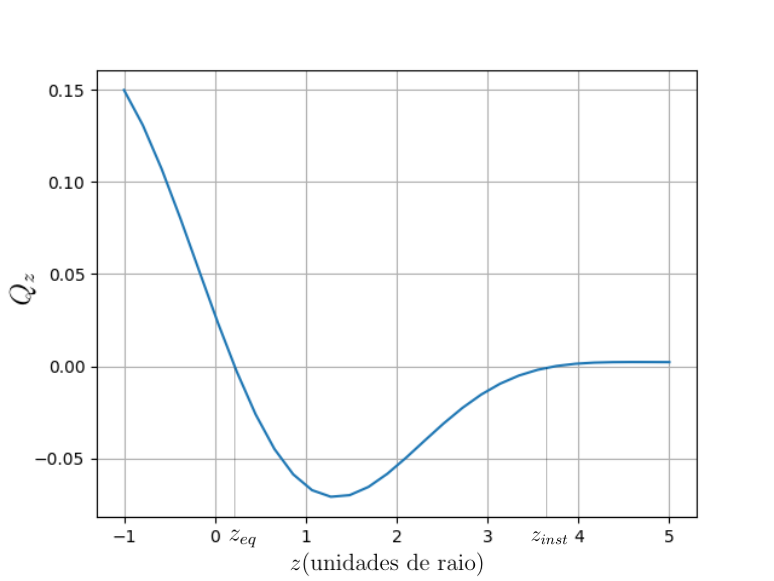
\includegraphics[scale=.35]{../Qz_tipico}}
        \end{picture}

        \begin{picture}(320,250)
        \put(160,353){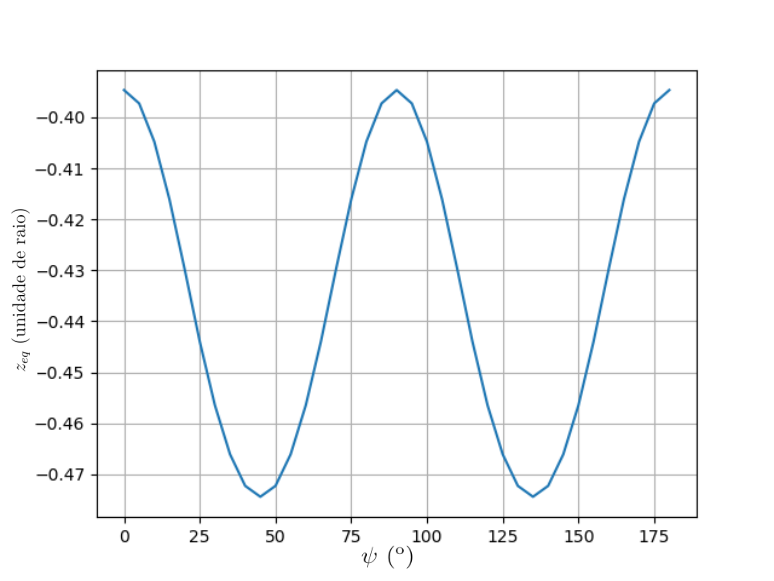
\includegraphics[scale=.36]{../zeq_psi_ast25II}}
        \end{picture}

    \end{center}

\end{frame}

%%%%%%%%%%%%%%%%%%%%%%%%%%%%%%%%%%%%%%%%%%%%%%%%%%%%%%%%%%%%%%%%%%%%%%%%%%%%%%%%%%%%%%%%%%%%%%%%%

\begin{frame}[fragile]{Resultados da simulação do experimento}

    \begin{center}
        Usando as posições de equilíbrio, calculamos as derivadas do fator de eficiência nas direções $\rho$ e $\phi$, e temos assim o ângulo da posição de equilíbrio.

        Variando o parâmetro de astigmatismo, usamos uma função erro para determinar qual conjunto de pontos numéricos tem maior verossimilhança com os dados experimentais. A função erro é definida como:

        \begin{equation}
        E(A_{ast})=\sum \limits_i \big{[} \phi_i^{exp} - \phi_i^{sim}(A_{ast}) \big{]}^2.
        \end{equation}

    \end{center}

\end{frame}

\begin{frame}[fragile]{Resultados da simulação do experimento}

    \begin{center}

        A seguir, dois exemplos de conjuntos de pontos teóricos com paprâmetros de astigmatismo diferentes ($A_{ast}=0$ na esquerda e $A_{ast}=0.36$ na direita):

        \begin{picture}(310,250)
        \put(-10,100){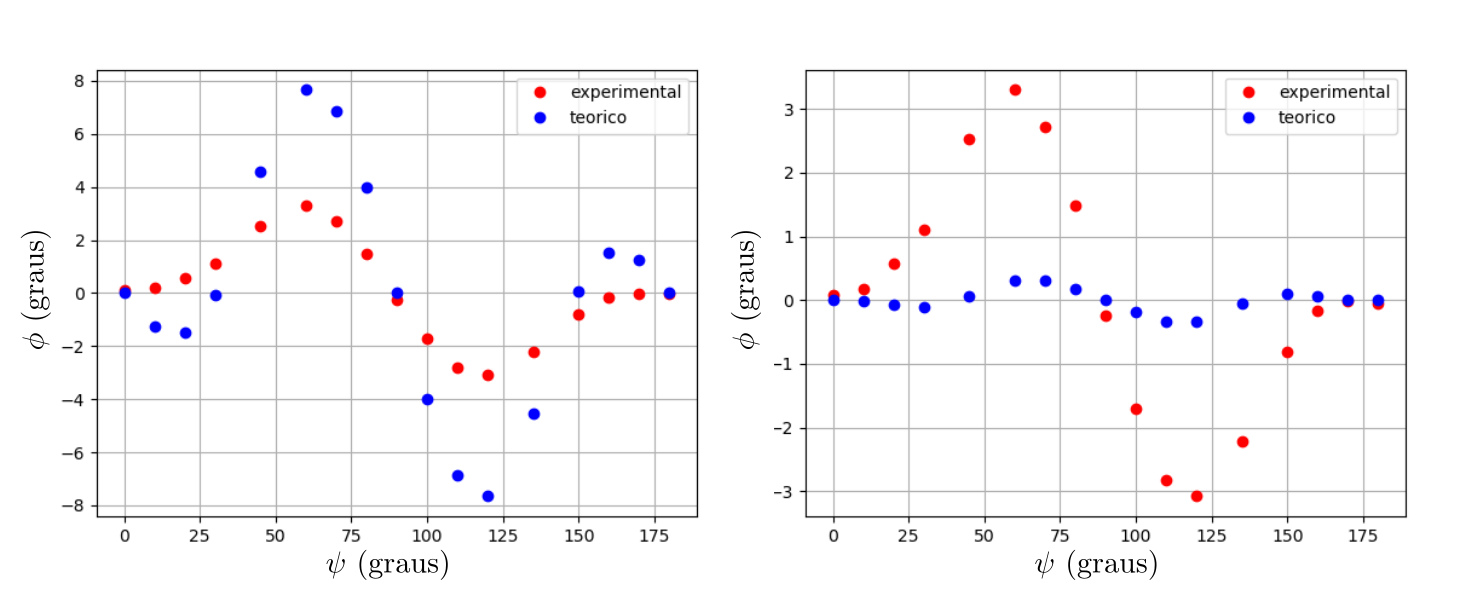
\includegraphics[scale=.38]{../Kphi_rho_Aast_dupla}}
        \end{picture}

    \end{center}

\end{frame}

\begin{frame}[fragile]{Resultados da simulação do experimento}

    \begin{center}

        O gráfico da função erro pelo parâmetro de astigmatismo apresenta um mínimo em $A_{ast}=0.24$, que corresponde ao valor mais provável do parâmetro de astigmatismo:

        \begin{picture}(310,250)
        \put(70,100){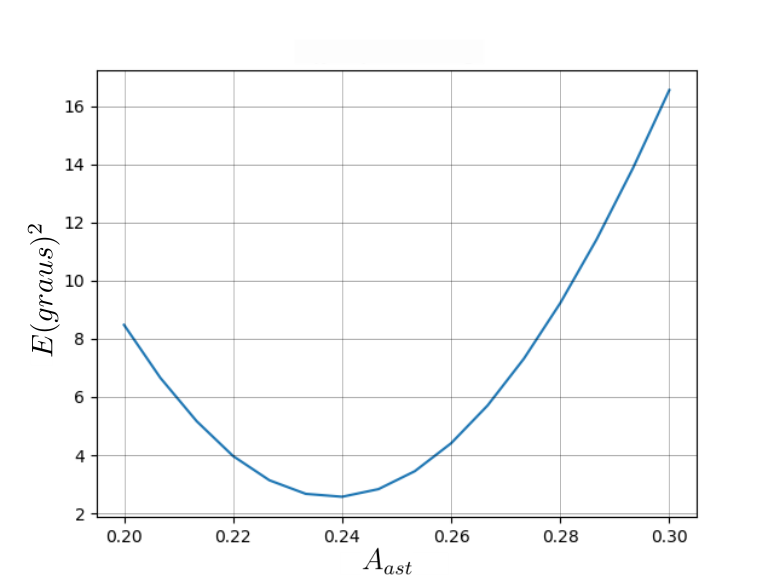
\includegraphics[scale=.38]{../erro_astigII}}
        \end{picture}

    \end{center}

\end{frame}

\begin{frame}[fragile]{Resultados da simulação do experimento}

    \begin{center}

        A seguir, mostramos o gráfico da posição angular $\phi$ em função do ângulo da placa de quarto de onda $\psi$ para o valor de $A_{ast}=0.24$:

        \begin{picture}(310,250)
        \put(70,100){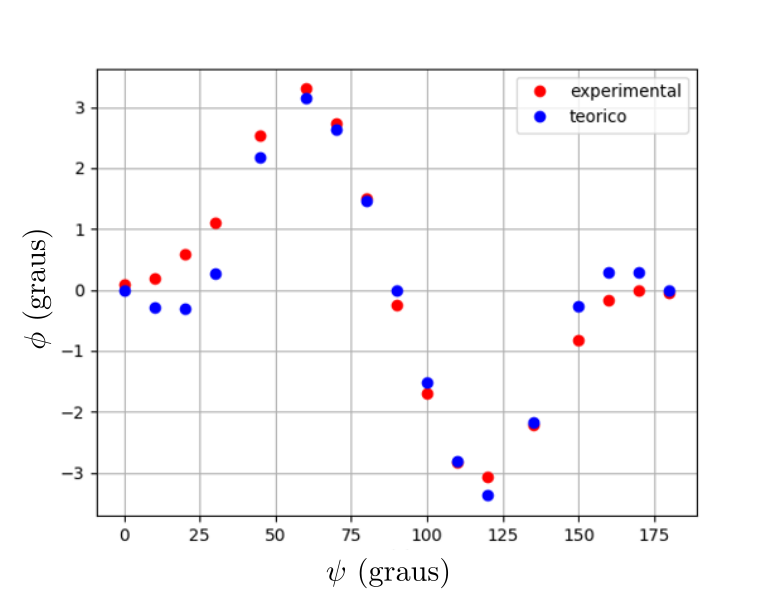
\includegraphics[scale=.38]{../Kphi_rho_Aast024III}}
        \end{picture}

    \end{center}

\end{frame}

%%%%%%%%%%%%%%%%%%%%%%%%%%%%%%%%%%%%%%%%%%%%%%%%%%%%%%%%%%%%%%%%%%%%%%%%%%%%%%%%%%%%%%%%%%%%%%%%%

\section{Caracterização do parâmetro de absorção da microesfera}

%%%%%%%%%%%%%%%%%%%%%%%%%%%%%%%%%%%%%%%%%%%%%%%%%%%%%%%%%%%%%%%%%%%%%%%%%%%%%%%%%%%%%%%%%%%%%%%%%

\begin{frame}[fragile]{Caracterização do parâmetro de absorção da microesfera}

  \begin{center}
      O que chamamos de parâmetro de absorção da microesfera é a parte imaginára do seu índice de refração. 

      O poliestireno é um material amplamente usado em experimentos de pinças óticas, e seu parâmetro de absorção é fornecido na literatura como $Im(n_{poli})=0.002$.

      Simulações com esferas grandes usadas e aprisionadas em laboratório não apresentaram qualquer posição de equilíbrio axial para esse valor quando o feixe incidente possui astigmatismo. Essa foi a motivação para o estudo da caracterização dessa grandeza, juntamente com o fato de haver uma forte dependência do fator de eficiência na direção $z$ com ela.

  \end{center}

\end{frame}

%%%%%%%%%%%%%%%%%%%%%%%%%%%%%%%%%%%%%%%%%%%%%%%%%%%%%%%%%%%%%%%%%%%%%%%%%%%%%%%%%%%%%%%%%%%%%%%%%

\begin{frame}[fragile]{Resultados da simulação do experimento}

    \begin{center}

        Os maiores valores de $Im(n_{poli})$ que apresentaram uma posição próxima ao eixo $z=0$ foram para $Im(n_{poli})=0.0004$, o que poderia indicar um equilíbrio com a força peso. O comportamento do fator de eficiência $Q_z$ em função de $z$ para vários raios está apresentado no gráfico a seguir:

        \begin{picture}(310,250)
        \put(-15,100){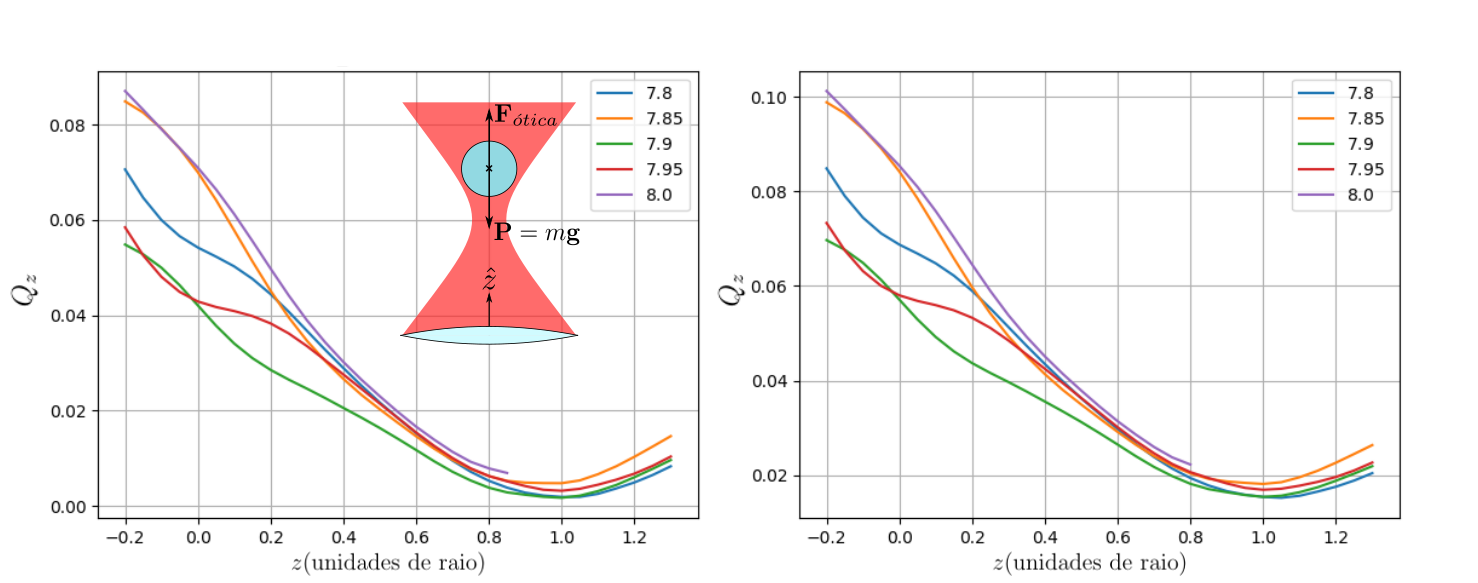
\includegraphics[scale=.38]{../Qz_z_1e-34II}}
        \end{picture}

    \end{center}

\end{frame}

%%%%%%%%%%%%%%%%%%%%%%%%%%%%%%%%%%%%%%%%%%%%%%%%%%%%%%%%%%%%%%%%%%%%%%%%%%%%%%%%%%%%%%%%%%%%%%%%%

\begin{frame}[fragile]{Caracterização do parâmetro de absorção da microesfera}

  \begin{center}
      Para voltar a observar posições de equilíbrio, podemos levar o parâmetro de astigmatismo a 0 e procurar parâmetros de abosorção que apresentem uma posição de equilíbrio próxima ao foco. Para fazer isso, o cálculo numérico para esferas menores é mais rápido, e o resultado é equivalente. Dessa forma, os valores de $n_{poli}$ tais que a posição de equilíbrio esteja ao menos 3 raios de de distância do plano focal estão representados pela parte preenchida do gráfico:

      \begin{picture}(310,250)
      \put(70,115){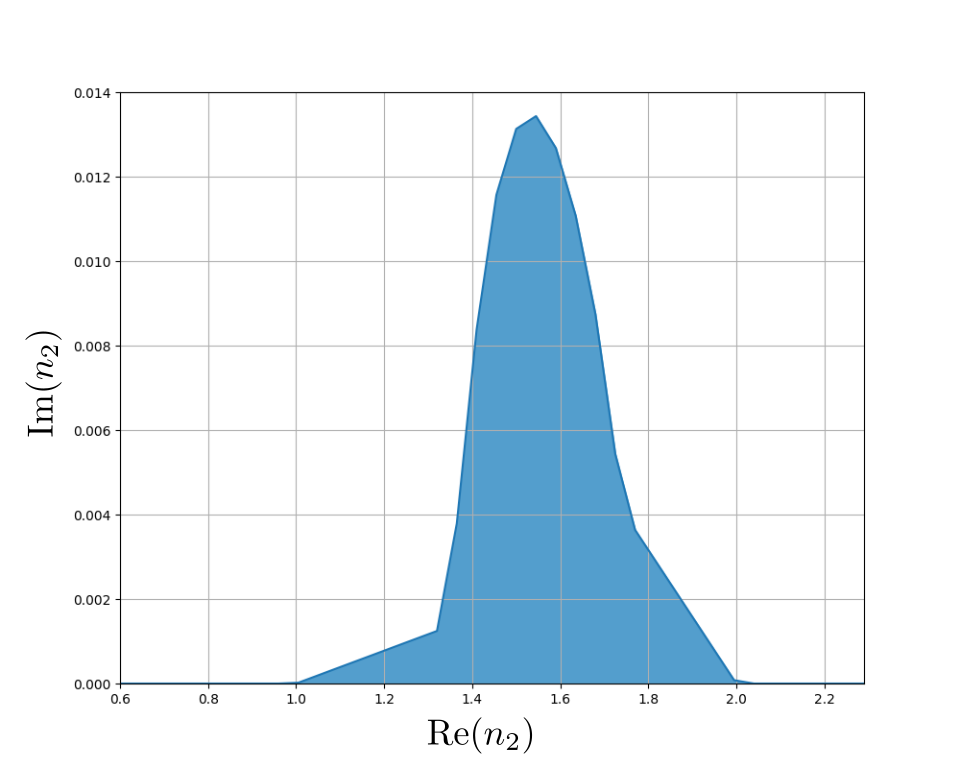
\includegraphics[scale=.23]{../Regiao_de_pincamentoII}}
      \end{picture}

  \end{center}

\end{frame}

%%%%%%%%%%%%%%%%%%%%%%%%%%%%%%%%%%%%%%%%%%%%%%%%%%%%%%%%%%%%%%%%%%%%%%%%%%%%%%%%%%%%%%%%%%%%%%%%%

\begin{frame}[fragile]{Caracterização do parâmetro de absorção da microesfera}

  \begin{center}
      Podemos propor um experimento para tentar caracterizar esse parâmetro. Como a força em $z$ tem uma dependência forte com $Im(n_{poli})$, podemos testar a condição de pinçamento observando as flutuações de energia potencial da pinça e calculando o tamanho da berreira potencial em $z$ que a esfera deve ultrapassar para sair do aprisionamento.

      Definimos o potencial efetivo para microesfera confinada no eixo $z$:
      %
      \begin{equation}
      V(z)=-\int\limits_{z_0}^{z} \frac{n_1P}{c} Q_z dz + V(z_0).
      \end{equation}

      O tamanho da barreira potencial é, então:
      %
      \begin{equation}
      \Delta=\int\limits^{z_{inst}}_{z_{eq}} Q_z \frac{dz}{a}.
      \end{equation}

  \end{center}

\end{frame}


%%%%%%%%%%%%%%%%%%%%%%%%%%%%%%%%%%%%%%%%%%%%%%%%%%%%%%%%%%%%%%%%%%%%%%%%%%%%%%%%%%%%%%%%%%%%%%%%%

\begin{frame}[fragile]{Caracterização do parâmetro de absorção da microesfera}

  \begin{center}
      A seguir, ilustramos as grandezas discutidas anteriormente. Em laranja, o fator de eficiência $Q_z(z)$, e em azul o potencial $V(z)$:

      \begin{picture}(310,250)
      \put(60,100){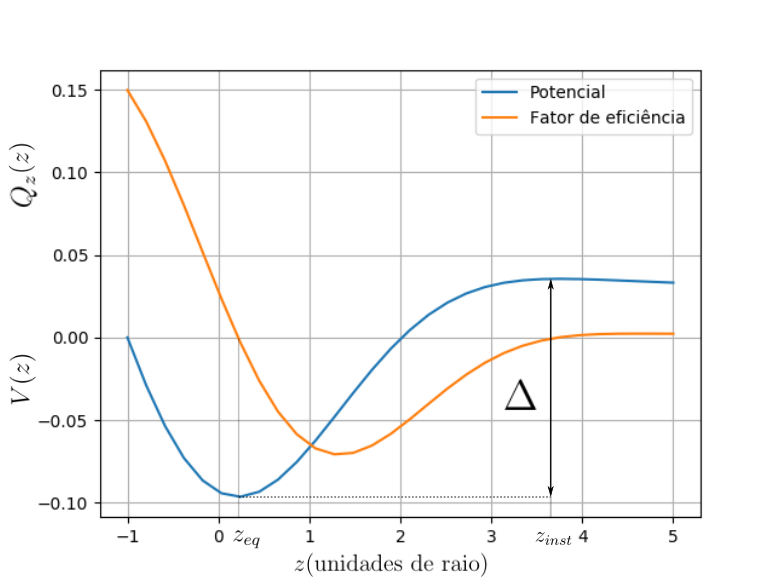
\includegraphics[scale=.4]{../potencial_qz}}
      \end{picture}

  \end{center}

\end{frame}

%%%%%%%%%%%%%%%%%%%%%%%%%%%%%%%%%%%%%%%%%%%%%%%%%%%%%%%%%%%%%%%%%%%%%%%%%%%%%%%%%%%%%%%%%%%%%%%%%

\begin{frame}[fragile]{Caracterização do parâmetro de absorção da microesfera}

  \begin{center}
      Fialmente, calculamos o tamanho da barreira potencial $\Delta$ para vários valores de $Im(n_{poli})$:
      %
      \begin{picture}(310,250)
      \put(60,100){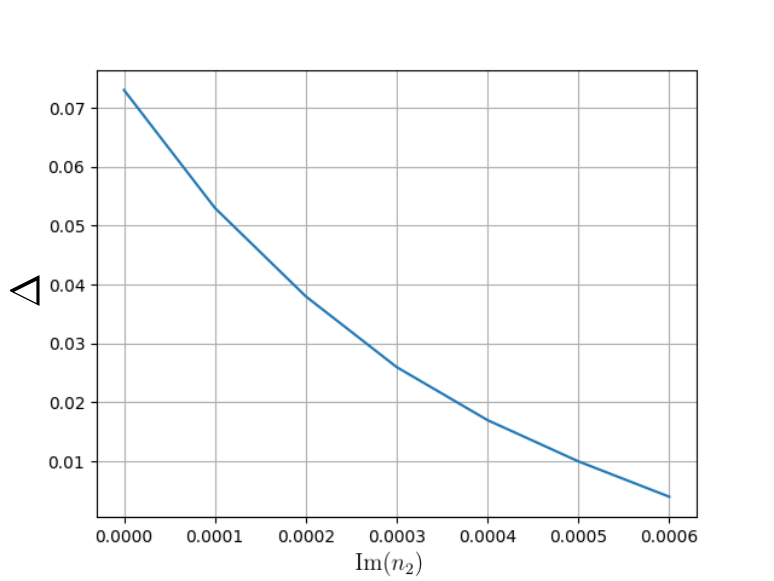
\includegraphics[scale=.4]{../Pot_EGII}}
      \end{picture}

  \end{center}

\end{frame}

%%%%%%%%%%%%%%%%%%%%%%%%%%%%%%%%%%%%%%%%%%%%%%%%%%%%%%%%%%%%%%%%%%%%%%%%%%%%%%%%%%%%%%%%%%%%%%%%%

\begin{frame}[fragile]{Caracterização do parâmetro de absorção da microesfera}

  \begin{center}

      Multiplicamos o valor de $\Delta$ por $(n_1 P a)/c$ para obter o valor da barreira potencial de fato.

      Podemos medir os valores máximos de flutuações de energia potencial da microesfera para tempos curtos, calibrando a constante elástica experimentalmente e observando as amplitudes de oscilação da microesfera. Ao diminuir a potencial $P$ do laser, podemos procurar o valor em que a microesfera escapa da pinça pelo eixo $z$.

      Medimos, então, a energia potencial máxima que a microesfera pode obter e a potencia do laser que permite a microesfera escapar. Portanto, podemos procurar o valor de $Im(n_{poli})$ que fornece uma barreira menor ou igual à energia da microesfera
 
  \end{center}

\end{frame}

%%%%%%%%%%%%%%%%%%%%%%%%%%%%%%%%%%%%%%%%%%%%%%%%%%%%%%%%%%%%%%%%%%%%%%%%%%%%%%%%%%%%%%%%%%%%%%%%%


%\begin{frame}{Animation}
%  \begin{itemize}[<+- | alert@+>]
%    \item \alert<4>{This is\only<4>{ really} important}
%    \item Now this
%    \item And now this
%  \end{itemize}
%\end{frame}



%{%
%\setbeamertemplate{frame footer}{---->Put footer in HERE}
%\begin{frame}[fragile]{Frame footer}
%    \themename defines a custom beamer template to add a text to the footer. It can be set via
%    \begin{verbatim}\setbeamertemplate{frame footer}{My custom footer}\end{verbatim}
%\end{frame}
%}

\section{Conclusão}

\begin{frame}[fragile]{Conclusão}

  \begin{center}

      \begin{itemize}

        \item bla


      \end{itemize}
 
  \end{center}

\end{frame}

%\begin{frame}[standout]
%  Questions?
%\end{frame}

\appendix


\end{document}
